\chapter{High throughput QTL mapping using correlated traits}
\thispagestyle{empty}
\label{chap:ctlmapping}

\emph{In this chapter we develop a new methodology to be used in quantitative genetics 
called Correlated Traits Locus (CTL) mapping, a method complementary to QTL mapping. 
Where QTL associates differences in mean, CTL, associate differences in correlation to 
genetic variation, i.e. CTL identify regions in the genome for which one genotype leads 
to correlated expression between a pair of traits, while the other genotype shows none 
(or significantly different) correlation.}

\null
\vfill

\begin{myexampleblock}{In press:}
  \authors{Danny Arends, Pjotr Prins, Yang Li, Lude Franke and Ritsert C. Jansen}\\
  \emph{CTL mapping}\\
  \bold{Draft}\\

  \authors{Danny Arends*, Harm-Jan Westra*, ... ,  Ritsert C. Jansen and Lude Franke}\\
  \emph{Cell-type specific eQTL analysis without the need to sort cells}\\
  \bold{Submitted}
\end{myexampleblock}

\newpage
\section{CTL mapping}
\subsection{Introduction}
  QTL mapping of a gene expression identifies regions in the genome at which different genotypes lead to differences in gene
  expression levels. In a similar fashion, abundance of thousands of proteins and metabolites can be measured to map protein 
  QTL (pQTL) and metabolite QTL (mQTL). 
  Deep sequencing, chromatin, and methylated DNA immunoprecipitation are just a few of the latest technologies that add to 
  the arsenal of tools available for the study of the genetic variation underlying quantitative phenotypes. Together, eQTL, 
  mQTL, and pQTL are referred to as xQTL \cite{Arends:2012}. Different xQTL can localize to confirm each other, for example, 
  with the \emph{A. thaliana} glucosinolate pathway \cite{Jansen:2009}. Such inference can lead to dissecting pathways and gene networks, 
  currently an active field of research \cite{Prins:2012}.

  Advances in QTL mapping focus on increasing QTL detection power and precision by using more and more advanced models to explain 
  observed variance. A higher amount of explained variance will result in a more reliable causal inference \cite{Li:2010}. Methods 
  developed to improve this explained variance are: Bayesian interval mapping, a framework to add prior knowledge \cite{Yandell:2007, 
  Hageman:2011}, Multiple QTL model (MQM) mapping tries to improves power by fitting a genetic model using backward elimination of 
  pre-selected genetic loci\rev{ }\cite{Jansen:1993, Arends:2010} and machine learning approaches, such as \rev{Random Forest} \cite{Bureau:2003}, 
  support vector machines (SVM), neural networks, and more recently vQTL mapping \cite{Valdar:2011} fall into this class of methods
  developed to improving power and attribute more variance to genetic factors.

  Another class of methods used in QTL mapping are the multivariate mapping approaches. These approaches combine variance information 
  from multiple traits to increase the number and significance of detected QTL. Methods like principal component analysis (PCA) and 
  differential expression (DE) analysis fall under the multivariate mapping methods. A review of many of these methods can be found 
  in Gilbert and le Roy \cite{Gilbert:2003}.

  Recently the field of analyzing differential networks has gained more and more attention. In these approaches the differences 
  between genetic networks are studied \cite{Fuente:2010,Horvath:2008}. Several approaches have been used to identify differential 
  correlations between experimental conditions for large-scale omics data sets using topological overlap \cite{Tesson:2010}. However 
  current approaches for detecting differential correlations only focus on the detection of differences in correlations between 
  two (or more) experimental conditions \cite{Fukushima:2013, Tesson:2010,Horvath:2008}. 

  We however believe that a major source of complementary information is available. Here, we present Correlated Traits Locus (CTL) 
  mapping, a method complementary to QTL mapping. Where QTL associates differences in mean, CTL, associate differences in correlation to 
  genetic variation, i.e. CTL identify regions in the genome for which one genotype leads to correlated expression between a pair of 
  traits, while the other genotype shows none (or significantly different) correlation. CTL information complements QTL information, 
  and provides insights into the genetic regulation of correlated traits, hidden in a traditional QTL mapping approach.
  
  %CTL mapping closes the gap between classical QTL mapping and differential network analysis by using the genotype as experimental 
  %conditions. At each genetic locus we divide our population in two genotype conditions, allowing us to map differential networks 
  %when only a single experimental condition is available. Added advantage of this approach is that CTL mapping allows us to detect 
  %which genetic locus is responsible for the difference in observed correlation.

  CTL mapping using the R/ctl package is performed in the same way as QTL mapping using the R/qtl \cite{Broman:2003, Arends:2010} 
  package. This means data and results from R/qtl are directly usable in the R/ctl package. The results section shows a small code 
  example, to show similarities between CTL mapping and QTL mapping using R/qtl.

\subsection{Calculating a CTL}
  A CTL is calculated at marker M by analyzing all possible phenotype-phenotype combinations. The input for the calculation is 
  the genotype of marker M and the phenotypes measured on the individuals. Rather than taking the mean phenotype value for each 
  of the genotypes, as is done with QTL mapping, correlation is calculated between p1 and p2 only for individuals with the 
  A allele, we do the same for the individuals with the B allele. In pseudo code:
\begin{verbatim}
    foreach p1 in Phenotypes
      foreach p2 in Phenotypes
        corA = cor(p1|A, p2|A)
        corB = cor(p1|B, p2|B)
\end{verbatim}
  In words: At marker M, split the individuals in two groups conditional on their genotypes. Now, for each pair of phenotypes 
  (p1 and p2) calculate the correlation between p1 and p2 using individuals with an A allele (corA) or with a B allele (corB). 
  When corA or corB is high it implies that p1 and p2 are regulated together conditional on the genotype.

  This calculation of differences in correlation using pairwise phenotypes conditional to genotype is repeated for all markers.

  For the sake of simplicity the example given here deals with a cross with only 2 alleles (A and B) CTL mapping however is not 
  limited to only two alleles (see the Discussion section).

  \subsubsection{Locating genetic markers acting on trait pairs}
  In itself, the difference in phenotype-phenotype correlations observed at specific markers is interesting. The correlation 
  suggests that the pair p1 and p2 are connected phenotypes. For molecular data p1 and p2 could be acting in tandem, they could 
  be in the same pathway, they could have the same regulator or they could be connected in some other way.
  Naturally, there is the possibility the correlation is there by chance, or by sequence polymorphisms \cite{Alberts:2007}.
  When the phenotypes p1 and p2 are highly correlated for both A and B, however, the genomic location at marker M may not be so
  meaningful in the context of genetics\rev{.}  But when correlate between expression levels varies significantly between genotype A 
  and B (e.g. $corA >> corB$), some form of regulation at marker M in genotype A in the genotype is implied.

  \subsubsection{Take the differential}
  Therefore, to calculate the CTL effect size, we add an extra step. CTL effect size is based on the difference between corAA and 
  corBB, i.e., the CTL effect is the delta of the correlations for the two genotypes AA and BB:

  $$ CTL = corAA - corBB $$

  Again, this CTL effect size is calculated for every genomic positions.  When at a certain genomic locations phenotypes T1 and T2 
  correlate highly in AA, but for BB do not (or significantly less) correlate there may be an effect of interest. This, in essence, 
  is a CTL. The CTL suggests the genomic location is operating on both traits in tandem for genotype (AA), but not in the other 
  genotype (BB). Therefore, a hidden factor X at the CTL location (M) may be involved controlling the correlation between the two 
  phenotypes.

  Finally, to correct for difference in sample size the full calculation reads for the CTL at markers M:
  
  $$  CTL = \frac{(Z(corAA) - Z(corBB))}{stderr} $$

  For calculation of Z and stderr see the section 'CTL analysis on N-genotypes' in the discussion.

  \subsubsection{Assigning significance}
  
  When scaling the difference between two Z-values using the standard error we obtain a T-statistic which follows a 
  normal distribution \cite{Biometry:1995} allowing us to calculate an exact p-value.

  This p-value still needs to be corrected for multiple testing by using a \rev{Bonferroni} correction or a multi-trait 
  permutation approach \cite{Breitling:2008a} to estimate the null distribution. When doing permutations in each round 
  the link between genotype and trait is broken, by redistributing at random genotypes to the individuals while not 
  allowing for duplicates. After 10.000+ permutations each CTL score is transformed into a p-value.

  Observing that a trait might show many other traits with a CTL at a marker we can also use an alternative approach: 
  Don't assign significance to the individual trait-trait connections, but summarize the effect across all traits, 
  then use Quantile-Based Permutation Thresholds \cite{Neto:2012}. Using this approach for CTL mapping will add power 
  to detect sets of co-localizing CTLs, but will obscure the individual trait-trait connections.

  When CTL scores observed in real data are higher than any CTL score obtained during permutation a Generalized 
  Pareto Distribution (GPD) is used to estimate the extreme tail of the null distribution \cite{Knijnenburg:2009}, 
  this allows likelihood estimates for the extreme scores observed to be estimated.
  
  \begin{figure}[h!]
  \centering
  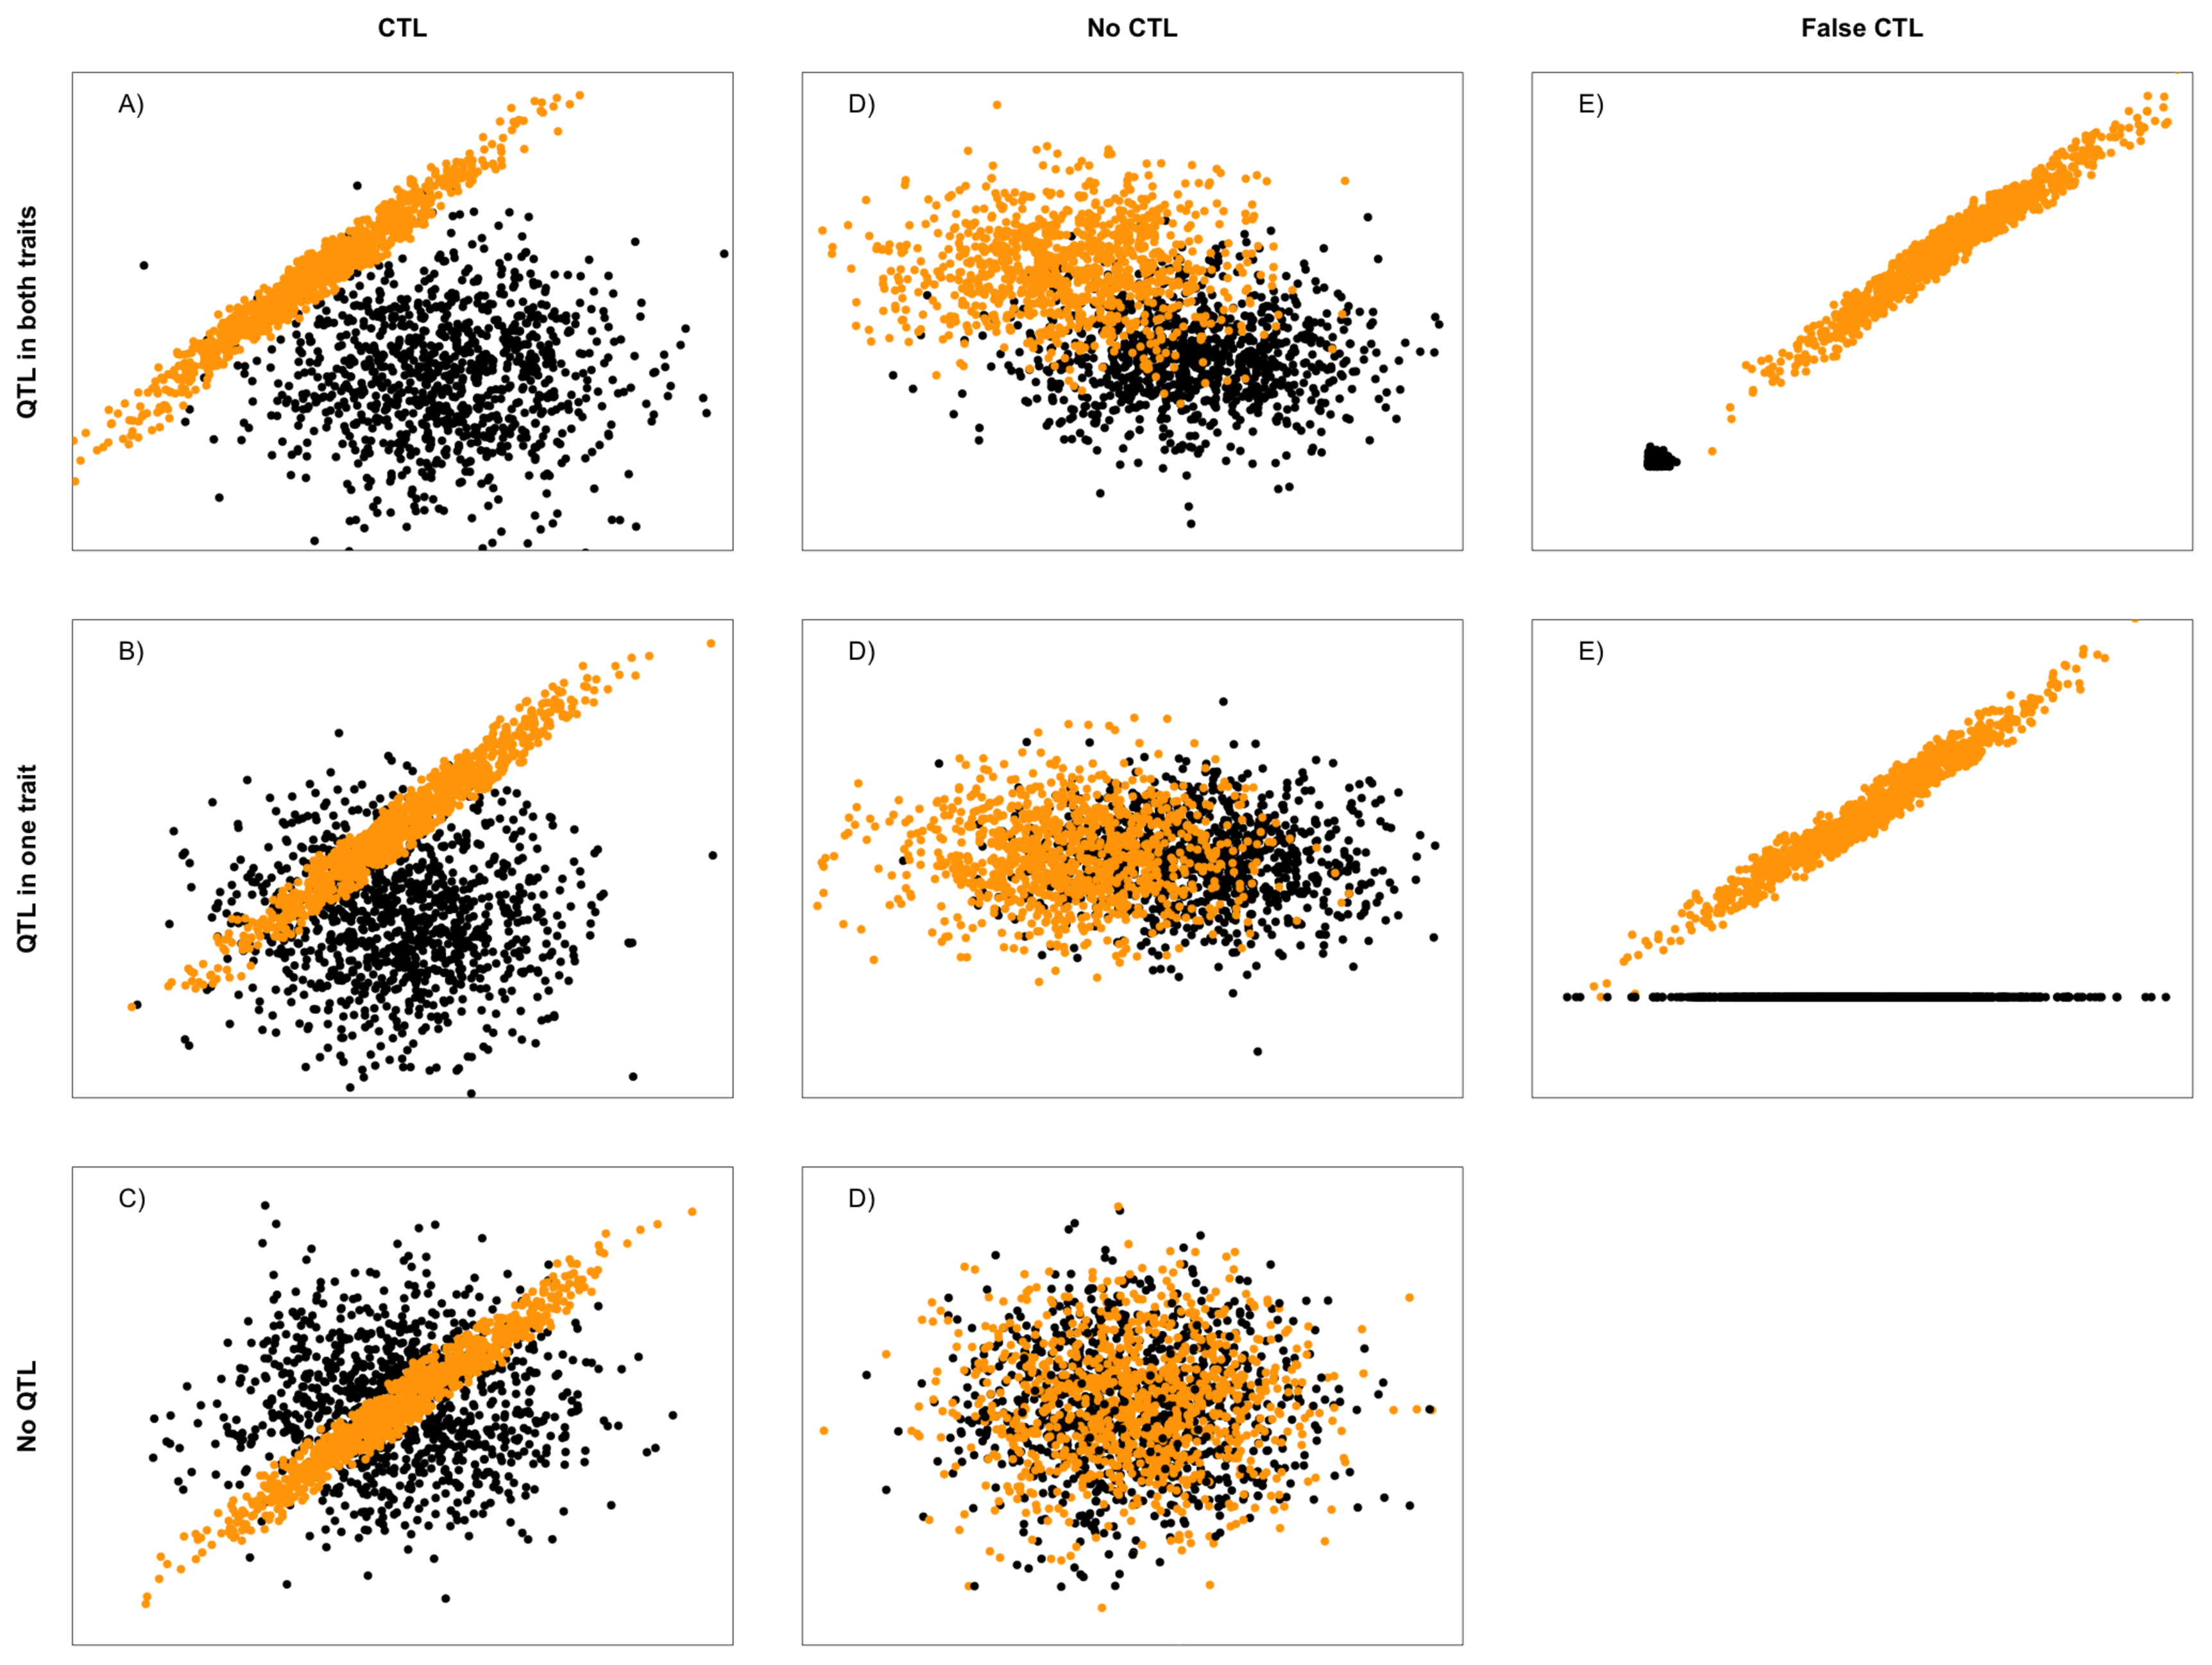
\includegraphics[width=0.9\textwidth]{eps/image_4_1.eps}
  \caption[CTLs.]{QTL and CTL analysis of two traits: a schematic of possible scenarios at a given marker. A trait can 
          have a QTL or no QTL at the given marker: there are four possible combinations in QTL analysis with two traits. 
          The trait pair can also have a CTL or no CTL and in the combined QTL and CTL analysis: the total number of possible 
          combinations is eight. Three additional scenarios refer to special cases when one trait or both traits are not 
          expressed in one genotype. For sake of simplicity it is assumed in this figure that there are two genotypes only, 
          e.g. as in a BC or RIL population. [We also ignore possible info on \emph{cis}- and \emph{trans}-mapping for the moment]}
          \label{fig:ctls}
  \end{figure}

  \subsubsection{QTL and CTL analysis of two traits}
  
  To describe the possible relationships between QTL and CTL we generate the possible scenario's as in figure \ref{fig:ctls}.\\
  {\bf(A)} The two traits have a QTL and a CTL at the given marker (1 scenario). This example shows the extreme scenario when the traits are 
  well correlated in one genotype and entirely uncorrelated in the other. The locus affects both the mean and the correlation. They could 
  have a regulatory factor in common, the effect of which is detected in QTL and CTL analysis.\\
  {\bf(B)} The two traits have a CTL at the given marker, but only one trait has a QTL at that marker (2 scenarios).  The locus affects the 
  correlation, and the mean of one trait only. They could have a regulator in common in which case the latter trait is downstream of the other 
  trait: this can happen e.g. if the locus leads to functionally different transcripts at equal expression levels for the trait without QTL, 
  and this effect is propagated to the trait with (therefore) a QTL.\\
  {\bf(C)} The two traits have a CTL but no QTL at the given marker (1 scenario). This example shows the extreme scenario when the traits 
  are well correlated in one genotype and entirely uncorrelated in the other.  The locus affects the correlation only. They could have a 
  regulatory factor in common, the effect of which is detected in CTL analysis only: e.g. if the locus leads to co-regulated transcription 
  in one genotype only.\\
  {\bf(D)} The two traits have no CTL at the given marker  (4 scenarios).  The locus does not change the correlation, it change the mean 
  if one or both traits have a QTL. The example shows the extreme scenario when both traits have a QTL but are entirely uncorrelated: they 
  could be downstream of the same or a different factor at the given region.\\
  {\bf(E)} The two traits have a CTL at the given marker, but the trait values are at the noise level in one genotype for one or both 
  traits (3 scenarios). This expression at noise level for one trait could result from e.g. hybridization failure for one genotype. One 
  or both traits can have a possibly artificial QTL and the two traits have a possibly artificial CTL. The example shows the scenario 
  when only one trait has a QTL.

\subsection{Inference of hierarchical relationship between traits}
  \subsubsection{Using information of co-localized CTL and QTL}
  Observing a significant CTL between T1 and T2 means that there is a factor (e.g. genetic regulator) located underneath 
  the CTL peak influencing the correlation between T1 and T2. This information of shared genetic control, therefore, 
  indicates that T1 and T2 are involved in the same biological pathway \cite{Tesson:2010}.

  The absence of QTL in trait T1 and the presence of QTL in trait T2 indicate that T2 is downstream of T1 in the 
  hierarchical network. The reasoning is that the variation caused by a genetic factor in T2 (QTL) has not 
  propagated to T1 \cite{Jansen:2009}. The reserve situation can also happen: Presence of QTL in trait T1 and the 
  absence of QTL in trait T2 indicate that T2 is upstream of T1 in the hierarchical network.

  The presence of QTL in both traits X and Y further confirms that T1 and T2 are related in the same pathway, and it 
  even allows us to go from inferring hierarchical relationship to causality using methods such as conditional 
  correlation \cite{Schadt:2007, Li:2010}.

  It should be noted that the co-localized CTL information does not exclude the existence of intermediate factor(s) 
  e.g. Z,  between T1 and T2 in the pathway, although the relative strength of correlation provides us 
  information on the distance among them in the network, e.g. higher correlation can indicate a shorter distance 
  between T1 and T2 in the network.\\

  \subsubsection{Using information of co-localized CTLs}
  When the CTLxy of X and Y co-localizes with CTLxz of X and Z and CTLyz of Y and Z, these three traits are possibly 
  involved in the same network. The relative effect sizes of these CTLs can be used to infer the order of X, Y and Z
  in the hierarchical network. For example, when CTLxy and CTLyz are larger than CTLxz, we can conclude that they 
  follow the order of X-Y-Z in the network, i.e. Y is in between of X and Z.

  Additionally when a QTL shows two or more co-localizing CTL we discovered a set of possible downstream targets 
  for the QTL. Which, when sample sizes permit, can be further annotated using gene ontology \cite{GeneOntology:2000} or 
  untangled by using methods like hierarchical inference (this paper) or causal inference \cite{Schadt:2005, Li:2006} 
  to obtain en even more detailed view of genetic regulation within the set.

  \subsubsection{Visualizing CTL information}
  Information obtained by CTL mapping can be visualized in several different ways the author found the most accessible 
  representation is a user-customizable network view. User customization helps researchers to add their own and/or 
  literature information to a network allowing for a rich interpretation of the created network. Network generated from 
  CTL mapping can be visualized by software tools including Cytoscape \cite{Cytoscape:2010, Cytoscape:2003}.

  CTL information allows us to draw lines from traits via markers to other traits reconstructing the underlying genetic 
  wiring. To create hierarchical networks we transforming the significant CTLs into network edges. This is done by 
  using a user defined genome wide FDR and then only transforming significant trait-marker-trait interactions into a 
  .sif network file.
  
  \subsubsection{CTL analysis on N-genotypes}
  CTL mapping on crosses with more than two genotypes (e.g. F2 or 4-way) or CTL on GWAS data where SNPs are used to 
  for association mapping, involves a slightly different approach then outlined in the methods section. Here we 
  detail our method while we assume not two but $k$ genotypes. For each genotype $i$, a sample size of $n_{i}$ 
  individuals is available.

  When $k$ independent correlation coefficients are to be compared a Fisher's Z-transformation is applied to each 
  of the individual correlation coefficients ($R_{i}$):

  $$ Z_{i} = 0.5[\ln(1 + R_{i}) - \ln(1-R_{i})] $$

  To perform CTL mapping when three or more genotypes are present, one may evaluate the Chi-square test statistic
  \cite{Kullback:1959, Csiszar:2004}, this has the following null hypothesis ($H_{0}$): All correlation coefficients 
  are almost equal. The test statistic is then calculated summing over all $k$:

  $$ Chi^2 = \sum_{i=1}^{k}[(n_{i} - 3).Z_{i}^2] - \frac{[\sum_{i=1}^{k}(n_{i} - 3).Z_{i}]^2 }{ \sum_{i=1}^{k}(n_{i} - 3) } $$
  Where i = 1, 2, 3, .., k.\\
  
  The Chi-square test statistic has $(k-1)$ degrees of freedom, where $k$ is the number of genotypes. We transform \rev{the obtained p-value} by 
  using the -$\log_{10}$(p-value) and store the obtained LOD score for this trait-trait combination, then continue to 
  the next genetic marker.

  \subsubsection{Slope and Correlation}

  There exists a relationship between the slope of the regression line and the correlation:

  $$ cor = \beta * \frac{SD_{x}}{SD_{y}}$$

  From this formula we can see that there is no difference between using correlation and regression when the standard 
  deviation in x is equal to the standard deviation in y ($\frac{SD_{x}}{SD_{y}} ~= 1$). However when there is a 
  difference between the standard deviation ratio, correlation and slope have two different interpretations. Meaning 
  that observed slope differences should be interpreted as different phenomenon then difference in correlation.

  \begin{figure}[h!]
  \centering
  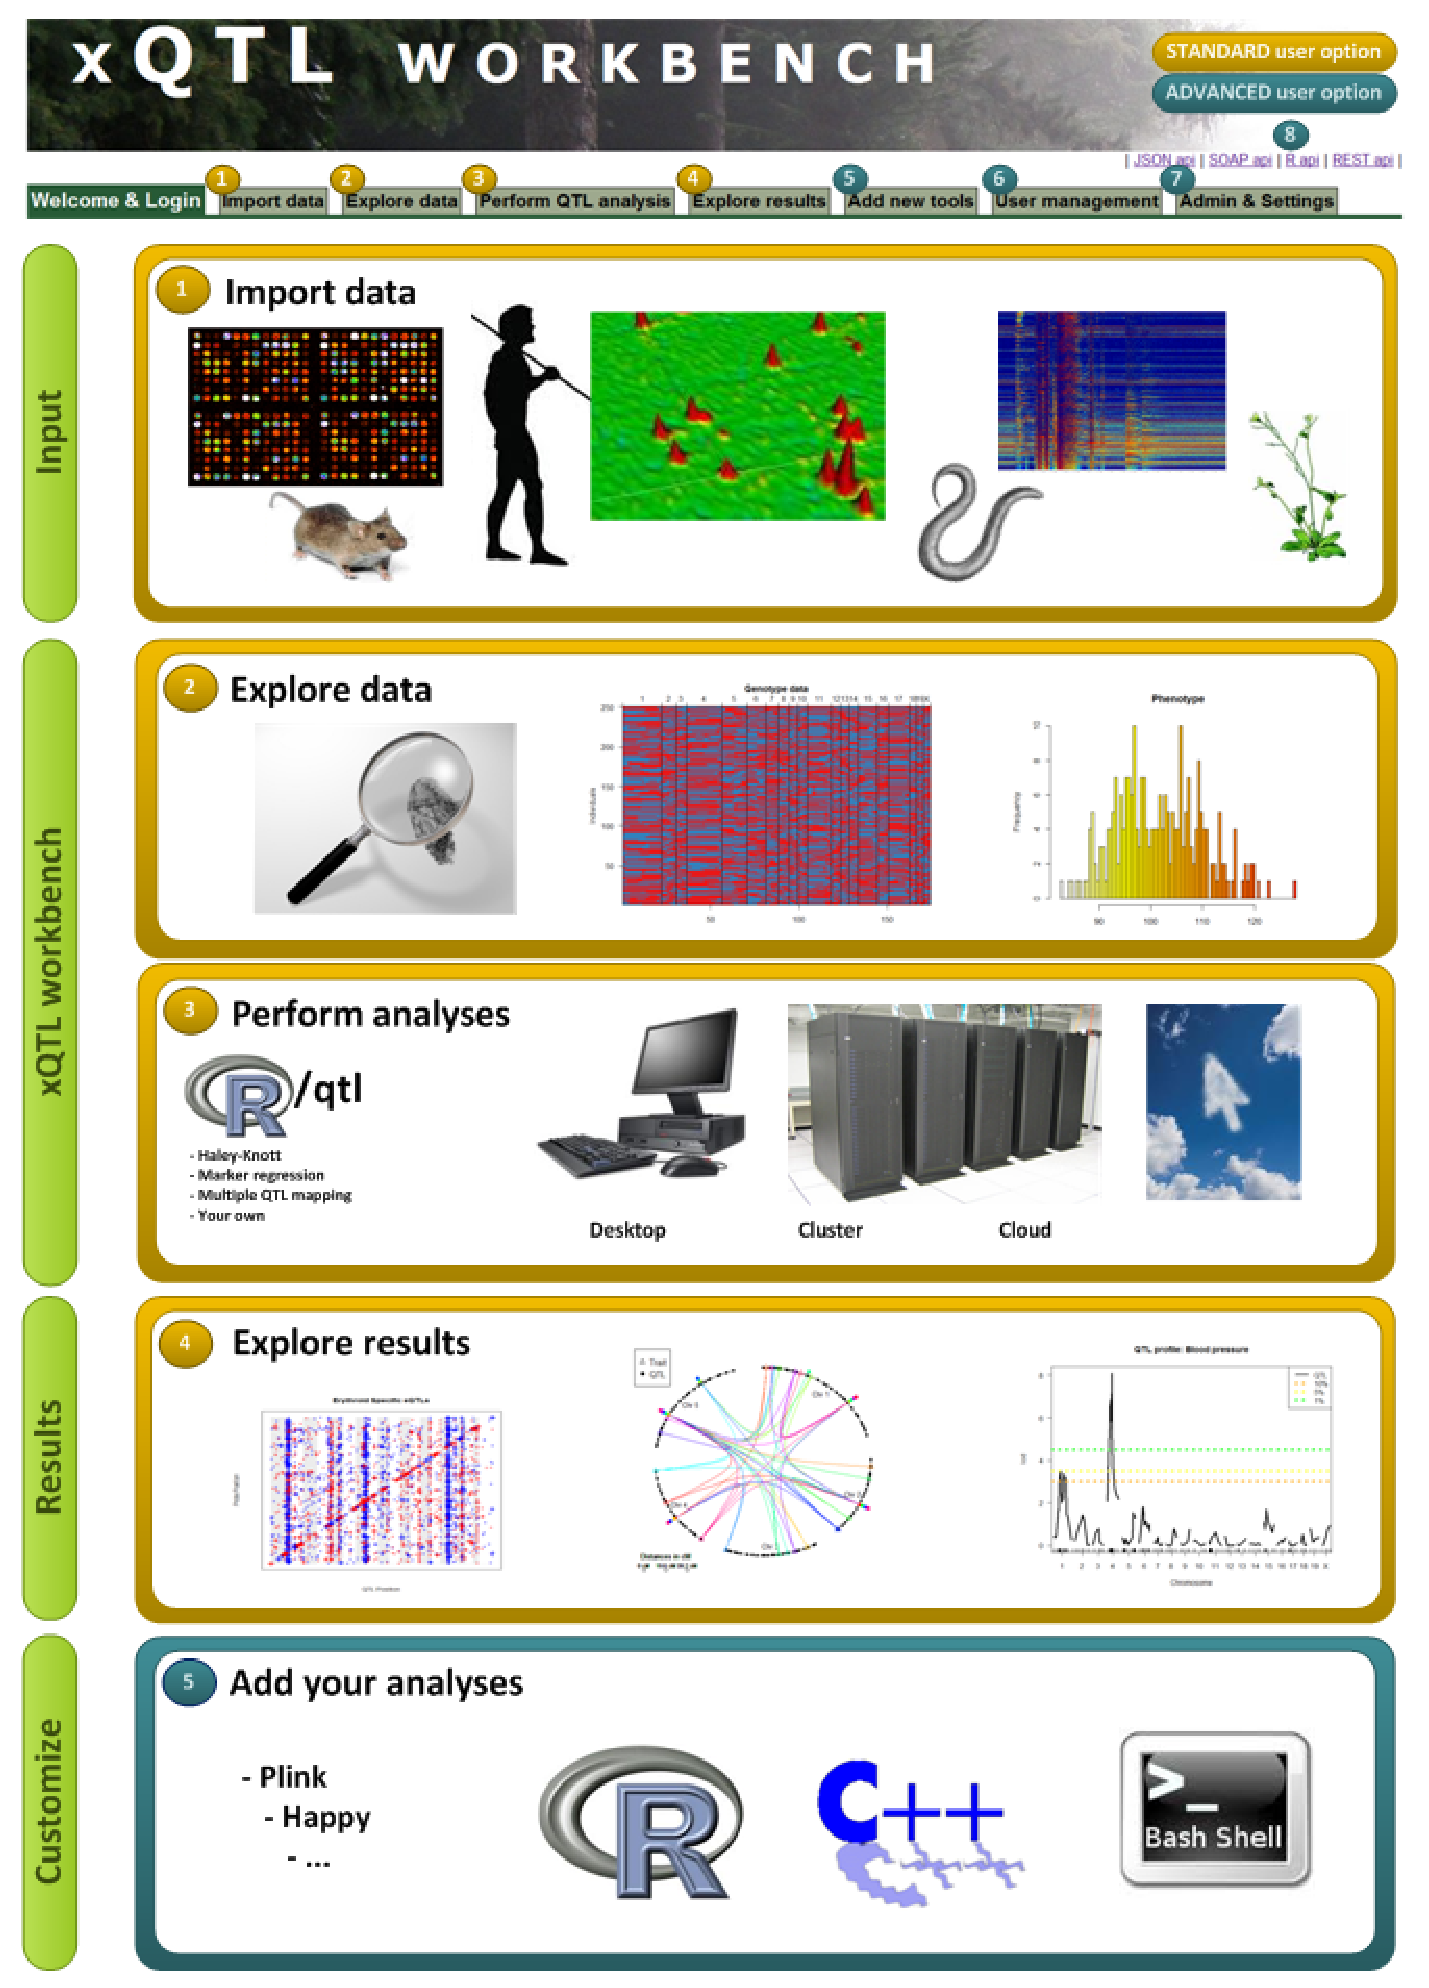
\includegraphics[width=0.9\textwidth]{eps/image_4_2.eps}
  \caption[Power analysis.]{Power analysis (using simulations done at a single marker) shows how 
                            much sample size is needed to obtain a given power at $alpha = 0.05$.\newline 
                            {\bf(left)} Increased effect sizes are detected with more power even at 
                            low sample sizes. To detect also small difference in correlation 
                            0.1 - 0.2 we need a large sample size (1000+).\newline
                            {\bf(right)} The closer the minor allele frequency is to 50\%, the more 
                            power to detect CTLs. This plot was created using a simulated effect size 
                            of 0.3 for all genotype ratio's. The effect of genotypes ratios on sample 
                            size shows that when ratios are close to 5\%, we need a three times larger 
                            sample size to detect the same effect. }
          \label{fig:fig4_2}
  \end{figure}

  \subsection{Power analysis}
  Using simulations the statistical power of our method can be determined when different effect sizes and/or genotype ratios 
  are encountered by the algorithm. A summary of the power analysis results are shown in Fig. \ref{fig:fig4_2}, and results 
  are discussed in the caption of this figure. 
  Code to simulate different effect sizes and genotype ratios is part of the CTL mapping R-package and can be used 
  to estimate (beforehand) the required sample size and/or the best breeding strategy to obtain the most power for detecting 
  CTL.

  \subsection{CTL power calculation applies to QTL and GWA}
  The power calculation that comes with the CTL method is a measure of the statistical power built into the experimental design 
  of an experiment. This applies not only to CTL, but has interesting implications for QTL and GWA studies in general. I.e., 
  the CTL power calculation is a measure of the statistical power of the experiment under analysis (QTL, CTL or GWA).


\section{Cell type specific eQTL mapping in human GWAS data}
\label{sec:cellspecificeqtl}
  Expression quantitative trait locus (eQTL) mapping on tissue, organ or whole organism data can detect associations that 
  are generic across cell types.  The number of available expression quantitative trait locus (eQTL) datasets from individual 
  cell types is limited because purifying cell types from mixtures is often challenging.  Since whole peripheral blood is 
  easily accessible and comprises many different cell-types (Figure \ref{fig:fig4_3}). Here we describe a new method to 
  focus upon specific cell types without first needing to sort  cells. We applied the method to whole blood data from 
  5,683 samples and demonstrate that SNPs associated with Crohn's  disease preferentially affect gene expression within neutrophils.
  \subsection{Background}

  In the past seven years, genome-wide association studies (GWAS) have identified thousands of genetic variants that are 
  associated with human disease \cite{Hindorff:2009}. The realization that many of the disease-predisposing variants are non-coding and that 
  single nucleotide polymorphisms (SNPs) often affect the expression of nearby genes (i.e. \emph{cis}-expression quantitative 
  trait loci; \emph{cis}-eQTLs)\cite{Lude:2011} suggests these variants have a predominantly regulatory function. Recent studies have shown 
  that disease-predisposing variants in humans often exert their regulatory effect on gene expression in a cell-type 
  dependent manner \cite{Brown:2013, Fairfax:2012, Fu:2012}. However, most human eQTL studies have used sample data obtained from mixtures of cell types (e.g. 
  whole blood) or a few specific cell types (e.g. lympoblastoid cell lines) due to the prohibitive costs and labor 
  required to purify subsets of cells from large samples (by cell sorting or laser capture micro-dissection). In addition, 
  the method of cell isolation can trigger uncontrolled processes in the cell, which can cause biases. In consequence, 
  it has been difficult to identify in which cell types these disease-associated variants exert their effect. 
  Here we describe a generic approach that deepens our interpretation of GWAS data to the level of individual cell types (Figure \ref{fig:fig4_4}). 

  \begin{figure}[h!]
  \centering
  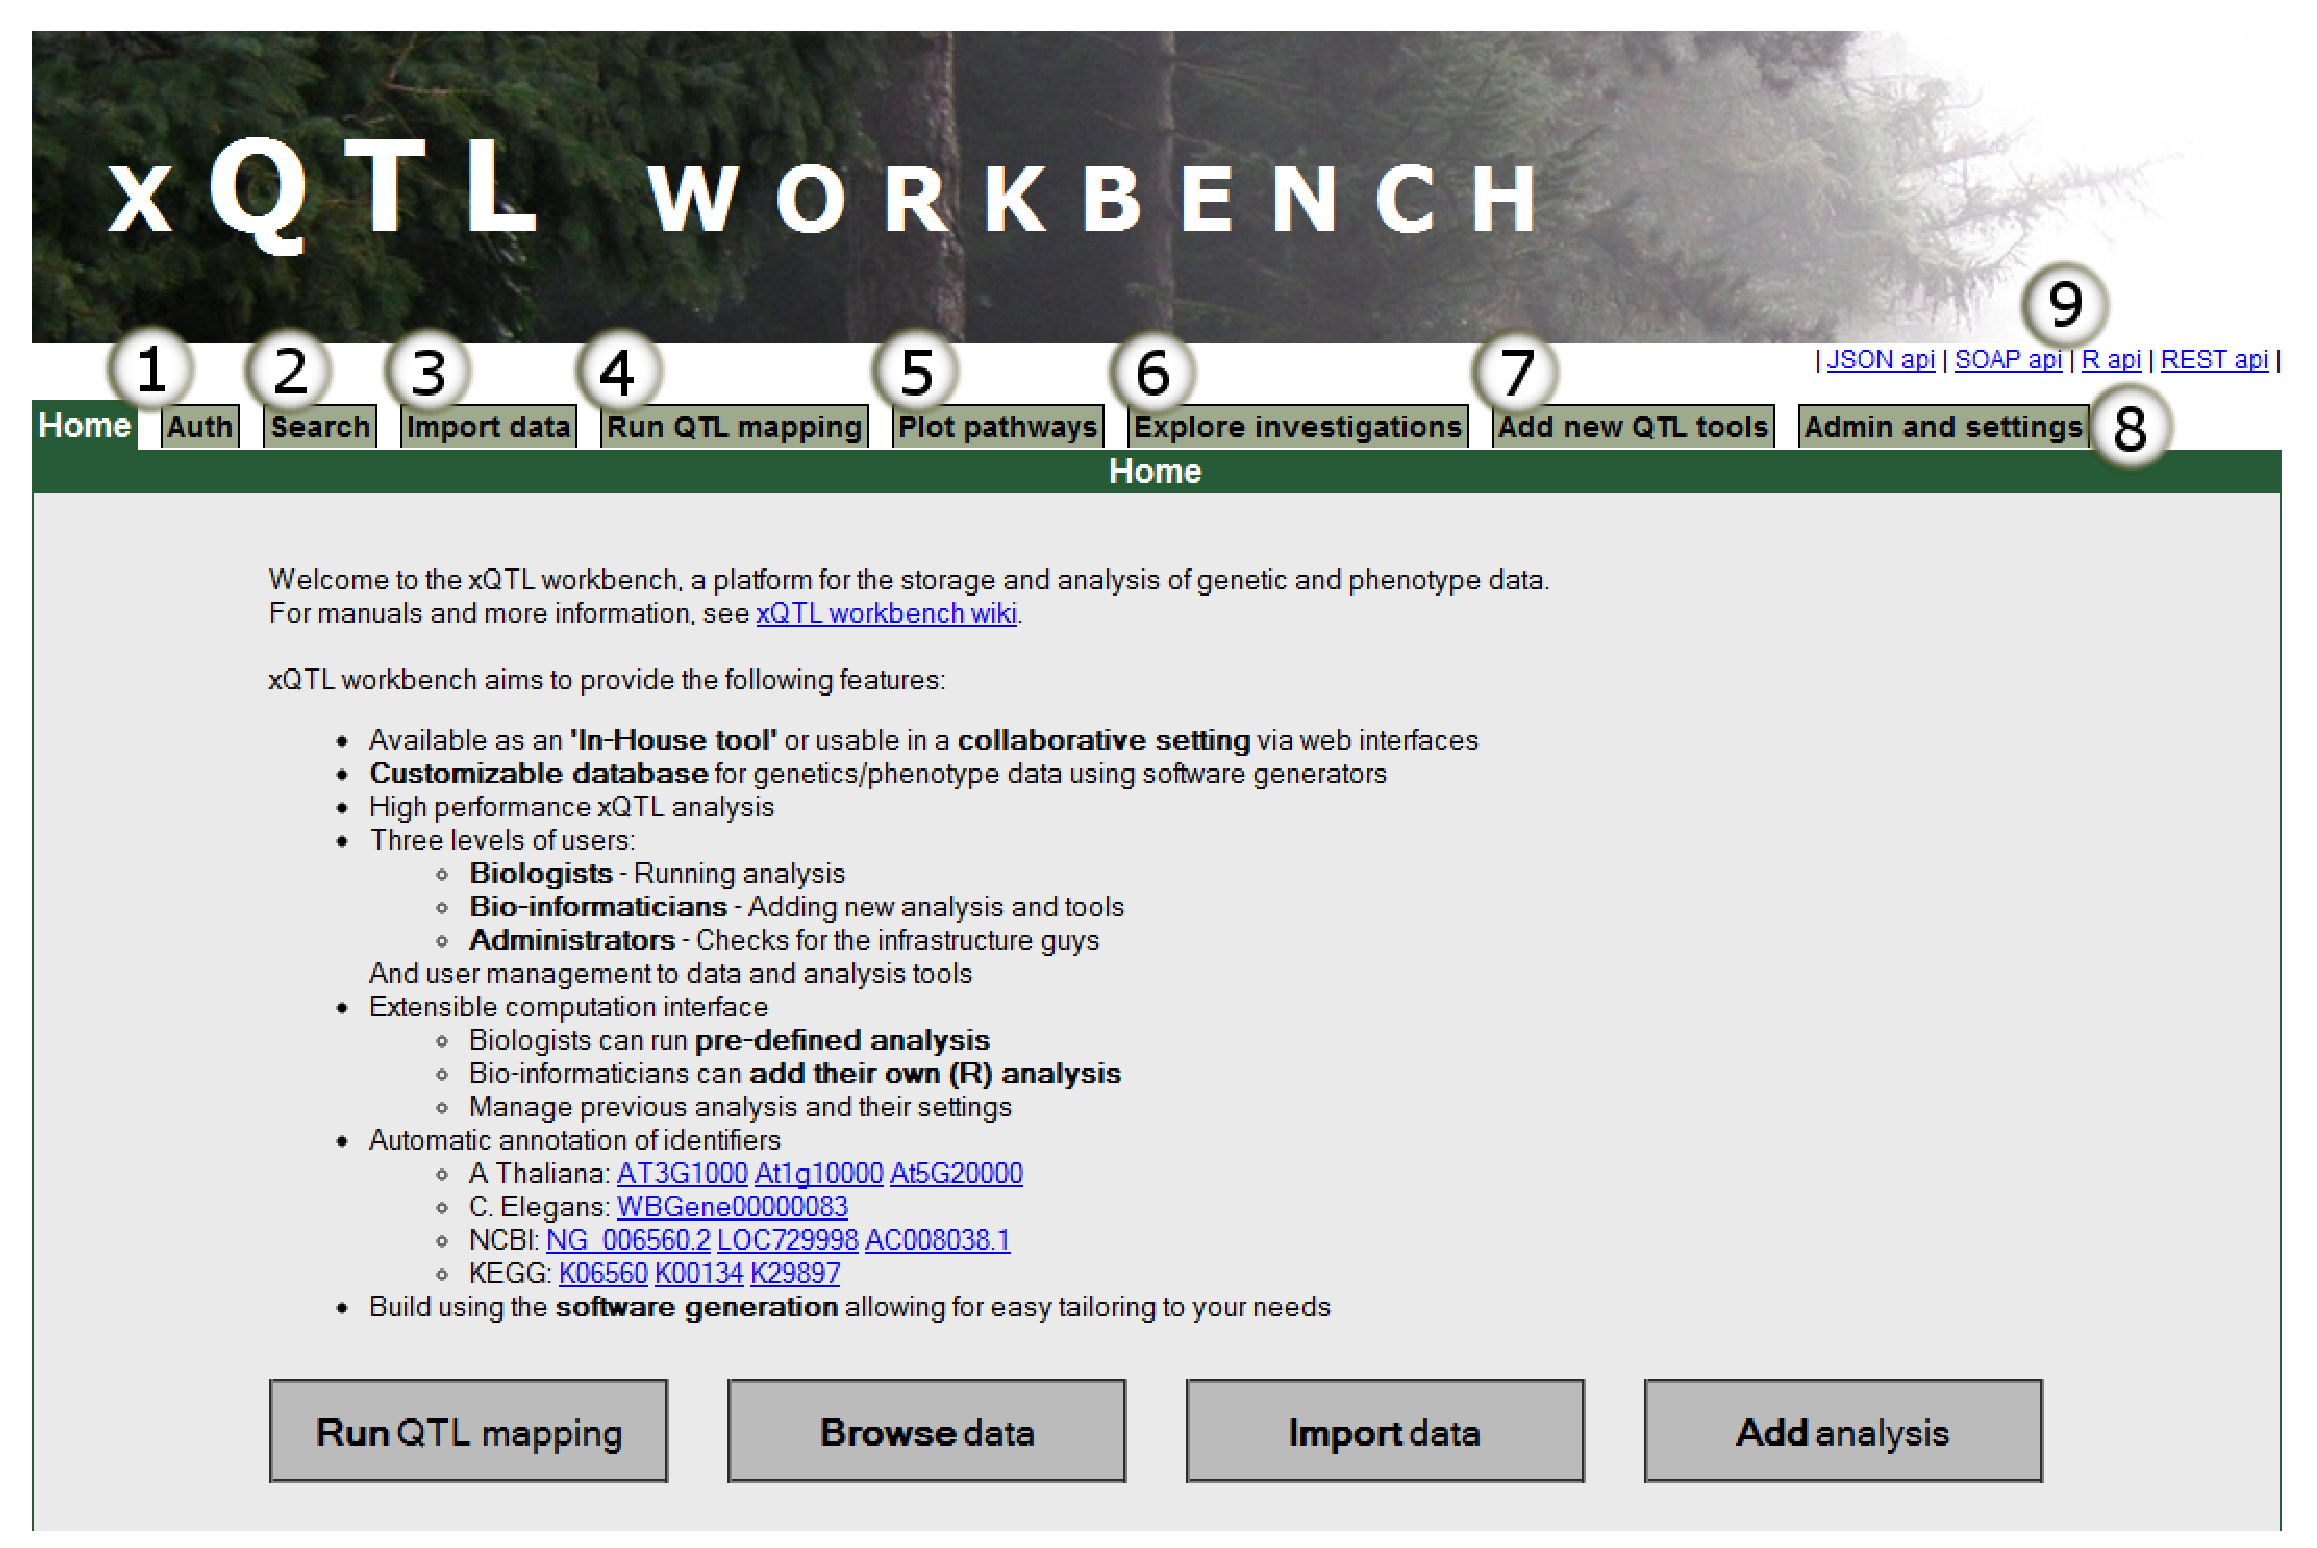
\includegraphics[width=0.9\textwidth]{eps/image_4_3.eps}
  \caption[Hematopoiesis overview]{Overview of cells involved in hematopoiesis. }
          \label{fig:fig4_3}
  \end{figure}

  \subsection{Method}
  Our strategy was to: (i) collect gene expression data from an entire tissue; (ii) predict the abundance of its constituent 
  cell types (i.e. the cell counts) by using expression levels of genes that serve as proxies for these cell types; (iii) run 
  an association analysis with a term for interaction between the SNP marker and the proxy for cell count to detect cell-type 
  mediated or -specific associations, and (iv) test whether known disease associations are enriched for SNPs that show the 
  cell-type-mediated or -specific effects on gene expression (i.e. eQTLs).

  We applied this method to 5,863 unrelated, whole blood samples from seven cohorts: EGCUT \cite{Metspalu:2004}, InCHIANTI 
  \cite{Tanaka:2009}, Rotterdam Study \cite{Hofman:2011}, Fehrmann \cite{Lude:2011}, SHIP-TREND 
  \cite{Teumer:2011}, KORA F4 \cite{Powell:2012, Mehta:2013}, and DILGOM \cite{Inouye:2010}. 
  Blood contains many different cell types that originate from either the myeloid (e.g. neutrophils and monocytes) or lymphoid lineage (e.g. B-cells and T-cells). 
  Even though neutrophils comprise ~62\% of all white blood cells, no neutrophil eQTL data have been published to date, because this cell type is particularly difficult 
  to purify or culture in the lab12. 

  For the purpose of illustrating our new cell-type specific analysis in the seven whole blood cohorts, we focused on neutrophils. 
  Direct neutrophil cell counts and percentages were only available in the EGCUT and SHIP-TREND cohorts, requiring us to infer 
  neutrophil percentages for the other five cohorts (Figure \ref{fig:fig4_4}). We used the EGCUT cohort as a training dataset to identify a list of 58 
  Illumina HT12v3 probes that correlated positively with neutrophil percentage (Spearman's correlation coefficient R > 0.55). 
  We then summarized the gene expression levels of these 58 individual probes into a single neutrophil percentage estimate, by 
  applying principal component analysis (PCA) and using the first principal component (see Supplementary Figure 1 for 
  confirmation of the accuracy of prediction in the SHIP-TREND cohort; Spearman R = 0.81). We then used this procedure in 
  the other cohorts to predict the neutrophil percentage.

  \subsection{Results}
  Identification of cell-type specific eQTLs in mixtures (e.g. whole peripheral blood) is most easily 
  understood when assuming an extreme situation where in half of all blood samples the proportion of 
  e.g. neutrophil granulocytes is very low, and in the other half of all blood samples this proportion 
  is actually high. If an eQTL of interest is not showing any effect in the samples with a very low 
  neutrophil granulocyte proportion, while showing a strong effect in the samples with a high proportion, 
  this suggests the eQTL is specific for neutrophil granulocytes. In order to apply this reasoning on 
  a whole blood dataset, the neutrophil percentage of each sample should be known and is used as a 
  covariate in a linear model that includes an interaction term (cell type percentage x genotype). 

  \begin{figure}[h!]
  \centering
  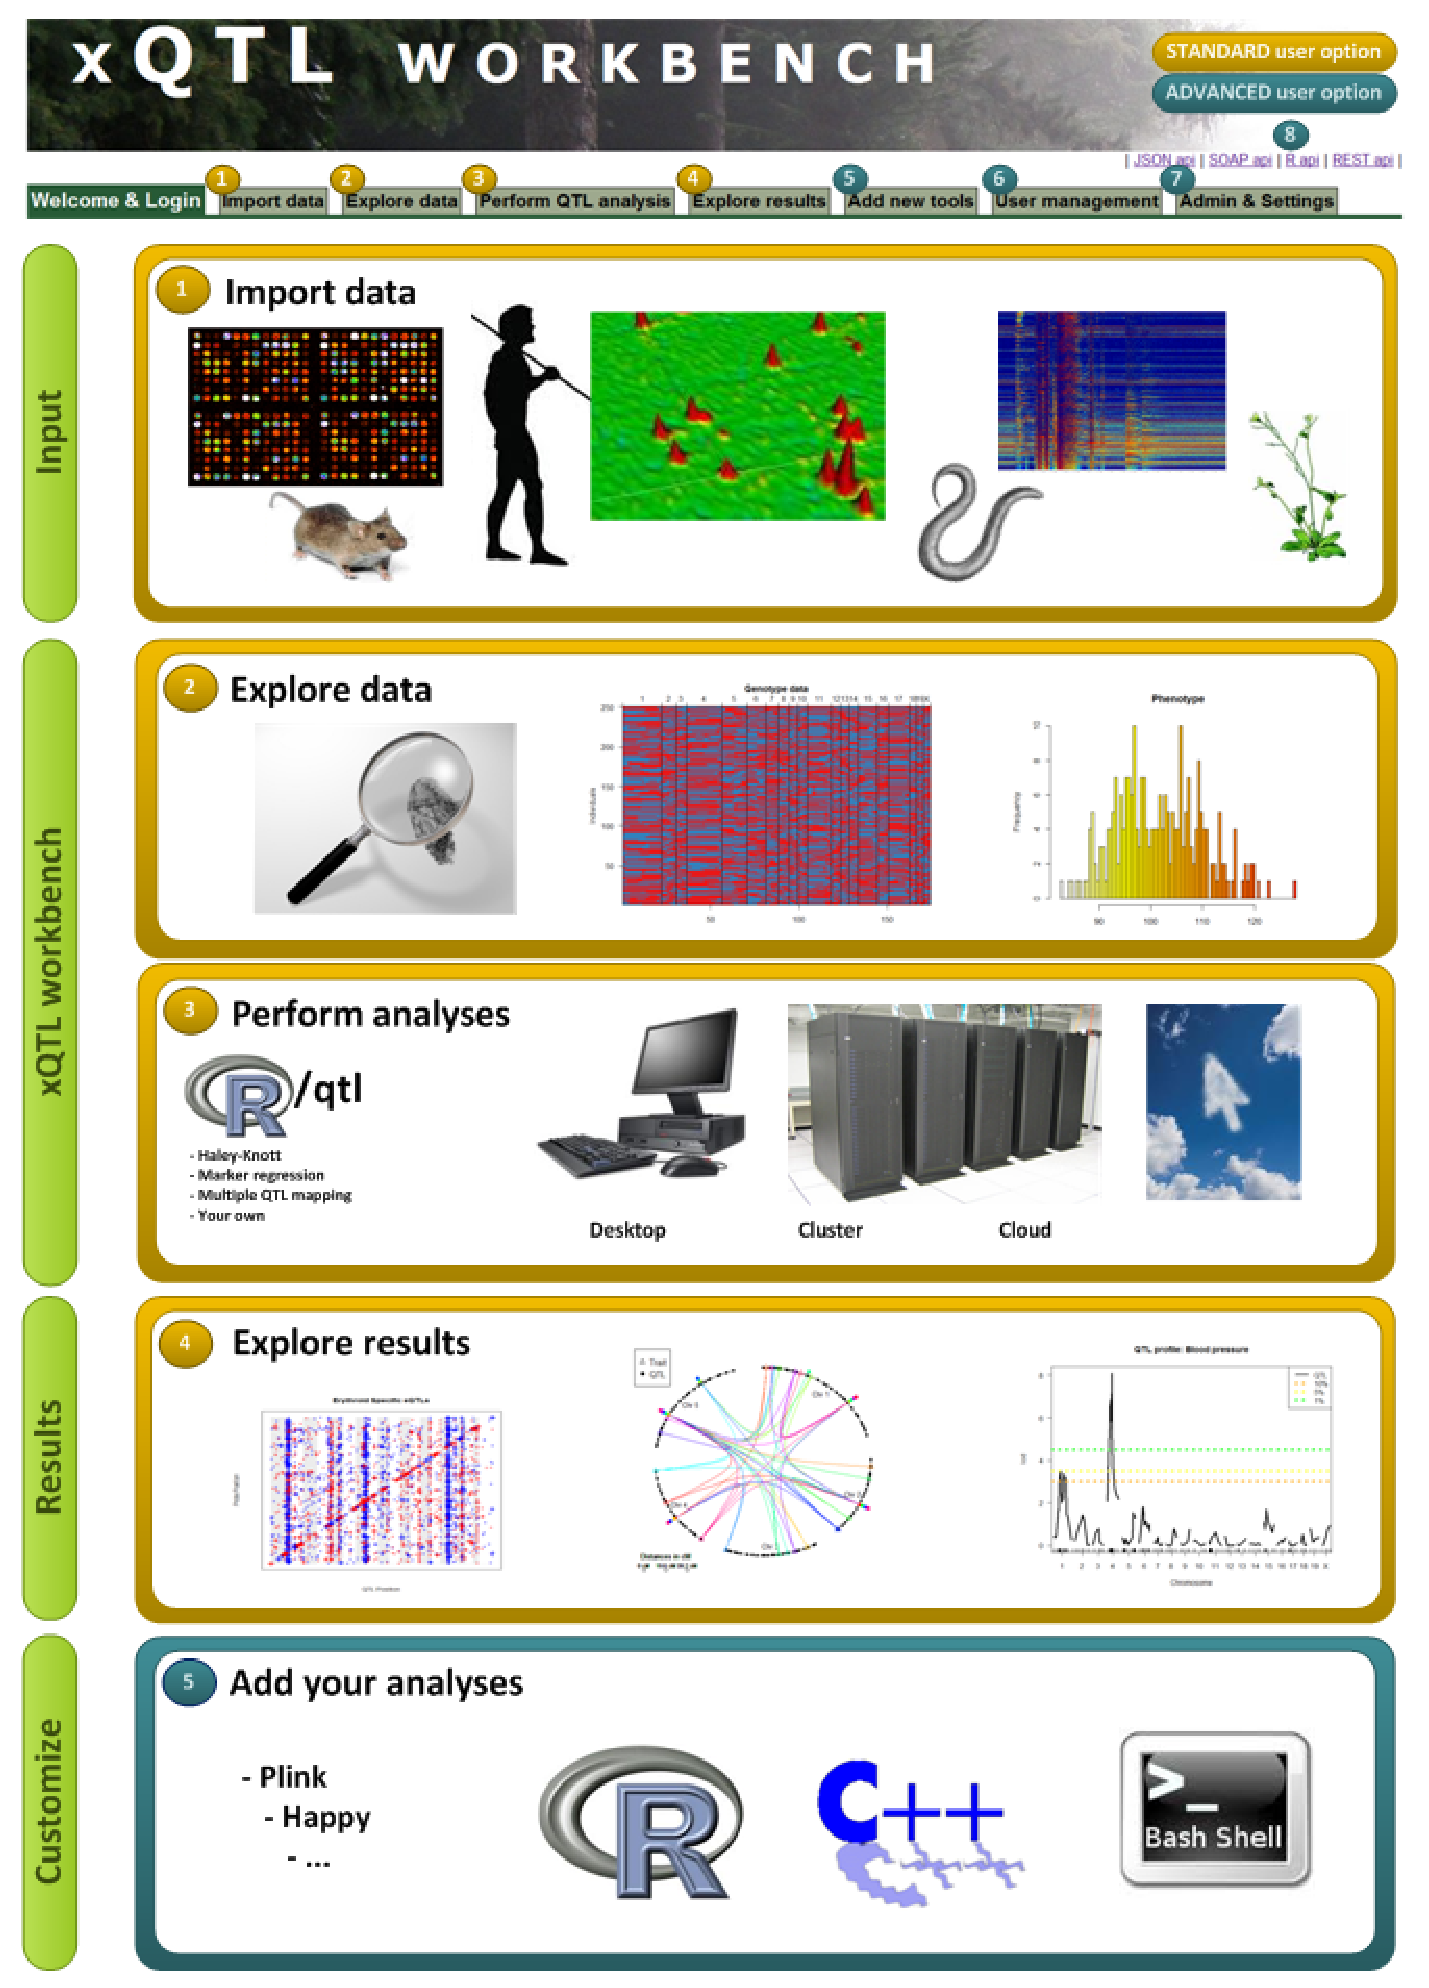
\includegraphics[width=0.9\textwidth]{eps/image_4_4.eps}
  \caption[Methods overview]{Overview of the method to detect cell type mediated \emph{cis}-eQTL in compound 
           tissues. A) Starting with a dataset that has cell count measurements, determine a set of 
           probes strongly positively correlating to the cell count measurements. Calculate the 
           correlation between these specific probes in the other datasets, and apply principal 
           component analysis to combine them into a single proxy for the cell count measurement. B) 
           Apply the neutrophil percentage predictor in the other cohorts. C) Use the proxy as a 
           covariate in a linear model with interaction term in order to distinguish cell type mediated 
           from non-cell type mediated \emph{cis}-eQTL effects, and classify each \emph{cis}-eQTL according to the 
           direction of the interaction effect.}
          \label{fig:fig4_4}
  \end{figure}

  Here we limit our analysis to 13,124 previously discovered \emph{cis}-eQTLs\cite{Westra:2013}, (although a genome-wide application of our method 
  might result in the detection of additional cell-type-specific \emph{cis}-eQTLs that we might have missed by assuming a generic 
  effect across cell types). We performed the eQTL association analysis with a term for interaction between the SNP marker 
  and the proxy for cell count within each cohort, followed by a meta-analysis (weighted for sample size) across all the 
  cohorts. We identified 1,117 \emph{cis}-eQTLs with a significant interaction effect (8.5\% of all \emph{cis}-eQTLs tested; false discovery 
  rate (FDR) < 0.05; 1,037 unique SNPs and 836 unique probes; Supplementary Tables 1 and 2). Out of the total number of \emph{cis}-eQTLs 
  tested, 909 (6.9\%) had a positive direction of effect, which indicates that these \emph{cis}-eQTLs show stronger effect sizes in 
  neutrophils ('neutrophil-mediated \emph{cis}-eQTLs'; 843 unique SNPs and 692 unique probes). Another 208 (1.6\%) had a negative direction 
  of effect (196 unique SNPs and 145 unique probes), indicating a stronger \emph{cis}-eQTL effect size in lymphoid cells ('lymphocyte-mediated 
  \emph{cis}-eQTLs'; since lymphocyte percentages are strongly negatively correlated with neutrophil percentages, Figure 1a). Overall, 
  the directions of the significant interaction effects were consistent across the different cohorts, indicating that our findings 
  are robust.

  We validated the neutrophil- and lymphoid-mediated associations we detected in six small, purified cell-type gene expression datasets (Figure \ref{fig:fig4_6}) 
  that had not been used in our meta-analysis. We generated new eQTL data from two lymphoid cell types (CD4+, n = 309 and CD8+ T-cells,
  n = 309) and one myeloid cell type (neutrophils, n = 114) and used previously generated eQTL data on two lymphoid 
  cell types (lymphoblastoid cell lines, n = 608, and B-cells, n = 283) and another myeloid cell type (monocytes, n = 282). As expected, 
  compared to \emph{cis}-eQTLs without a significant interaction term ('generic \emph{cis}-eQTLs', n = 12,007) the 909 neutrophil-mediated \emph{cis}-eQTLs did 
  indeed show very strong \emph{cis}-eQTL effects in both of the myeloid datasets (Wilcoxon P-value ≤ 4.9 x 10-31), 
  and small effect sizes in the lymphoid datasets. Coversely, the 208 lymphoid-mediated \emph{cis}-eQTLs had a pronounced effect in each of the 
  lymphoid datasets (Wilcoxon P-value ≤ 7.8 x 10-14; Figure \ref{fig:fig4_6}), while having small effect sizes in the myeloid datasets. These results 
  indicate that our method is able to reliably predict whether a \emph{cis}-eQTL is mediated by a specific cell type. Unfortunately, the cell 
  type that mediates the \emph{cis}-eQTL is not necessarily the one in which the \emph{cis}-gene has the highest expression, making it impossible to identify 
  of cell-type-specific eQTLs directly on the basis of expression levels.

  \begin{figure}[h!]
  \centering
  \includegraphics[width=0.9\textwidth]{eps/image_4_6.eps}
  \caption[Validation]{We validated the neutrophil and lymphoid mediated \emph{cis}-eQTL effects in four purified cell 
                       type datasets from the lymphoid lineage (B-cells, CD4+ T-cells, CD8+ T-cells and 
                       lymphoblastoid cell lines) and two datasets from the myeloid lineage (Monocytes and 
                       neutrophil granulocytes). Compared to generic \emph{cis}-eQTLs, large effect sizes are observed 
                       for lymphoid mediated \emph{cis}-eQTLs in lymphoid lineage cell types, while neutrophil mediated 
                       \emph{cis}-eQTL effects have large effect sizes specifically in the neutrophil datasets. These 
                       results indicate that our method is able to reliably predict whether a specific \emph{cis}-eQTL 
                       is mediated by cell type. }
          \label{fig:fig4_6}
  \end{figure}

  Myeloid and lymphoid blood cell types provide crucial immunological functions. Therefore, we assessed five immune-related diseases 
  for which genome-wide association studies previously identified at least 20 loci with a \emph{cis}-eQTL in our meta-analysis. We observed 
  a significant enrichment only for Crohn's disease (CD), (binomial test, one-tailed P = 0.002, Table \ref{tbl:tblDisease}): out of 49 
  unique CD-associated SNPs showing a \emph{cis}-eQTL effect, 11 (22\%) were neutrophil-mediated. These 11 SNPs affect the expression of 14 
  unique genes (ordered by size of interaction effect: IL18RAP, CPEB4, RP11-514O12.4, RNASET2, NOD2, CISD1, LGALS9, AC034220.3, SLC22A4, 
  HOTAIRM2, ZGPAT, LIME1, SLC2A4RG, and PLCL1). CD is a chronic inflammatory disease of the intestinal tract, and neutrophils are essential 
  for killing microbes that translocate through the mucosal layer of the intestine. The mucosal layer is affected in CD, but also in 
  monogenic diseases with neutropenia and defects in phagocyte bacterial killing, such as chronic granulomatous disease, glycogen storage 
  disease type I, and congenital neutropenia, leading to various CD phenotypes14. In addition, pharmacological interventions for the 
  treatment of CD have been developed to specifically target neutrophils, including Sagramostim15 and Natalizumab16. Our new analysis 
  shows clear neutrophil-mediated eQTL effects for many of the known CD genes, including the archetypal NOD2 gene, and our results 
  provide deeper insight into the role of neutrophils in CD pathogenesis.

  \begin{figure}[h!]
  \centering
  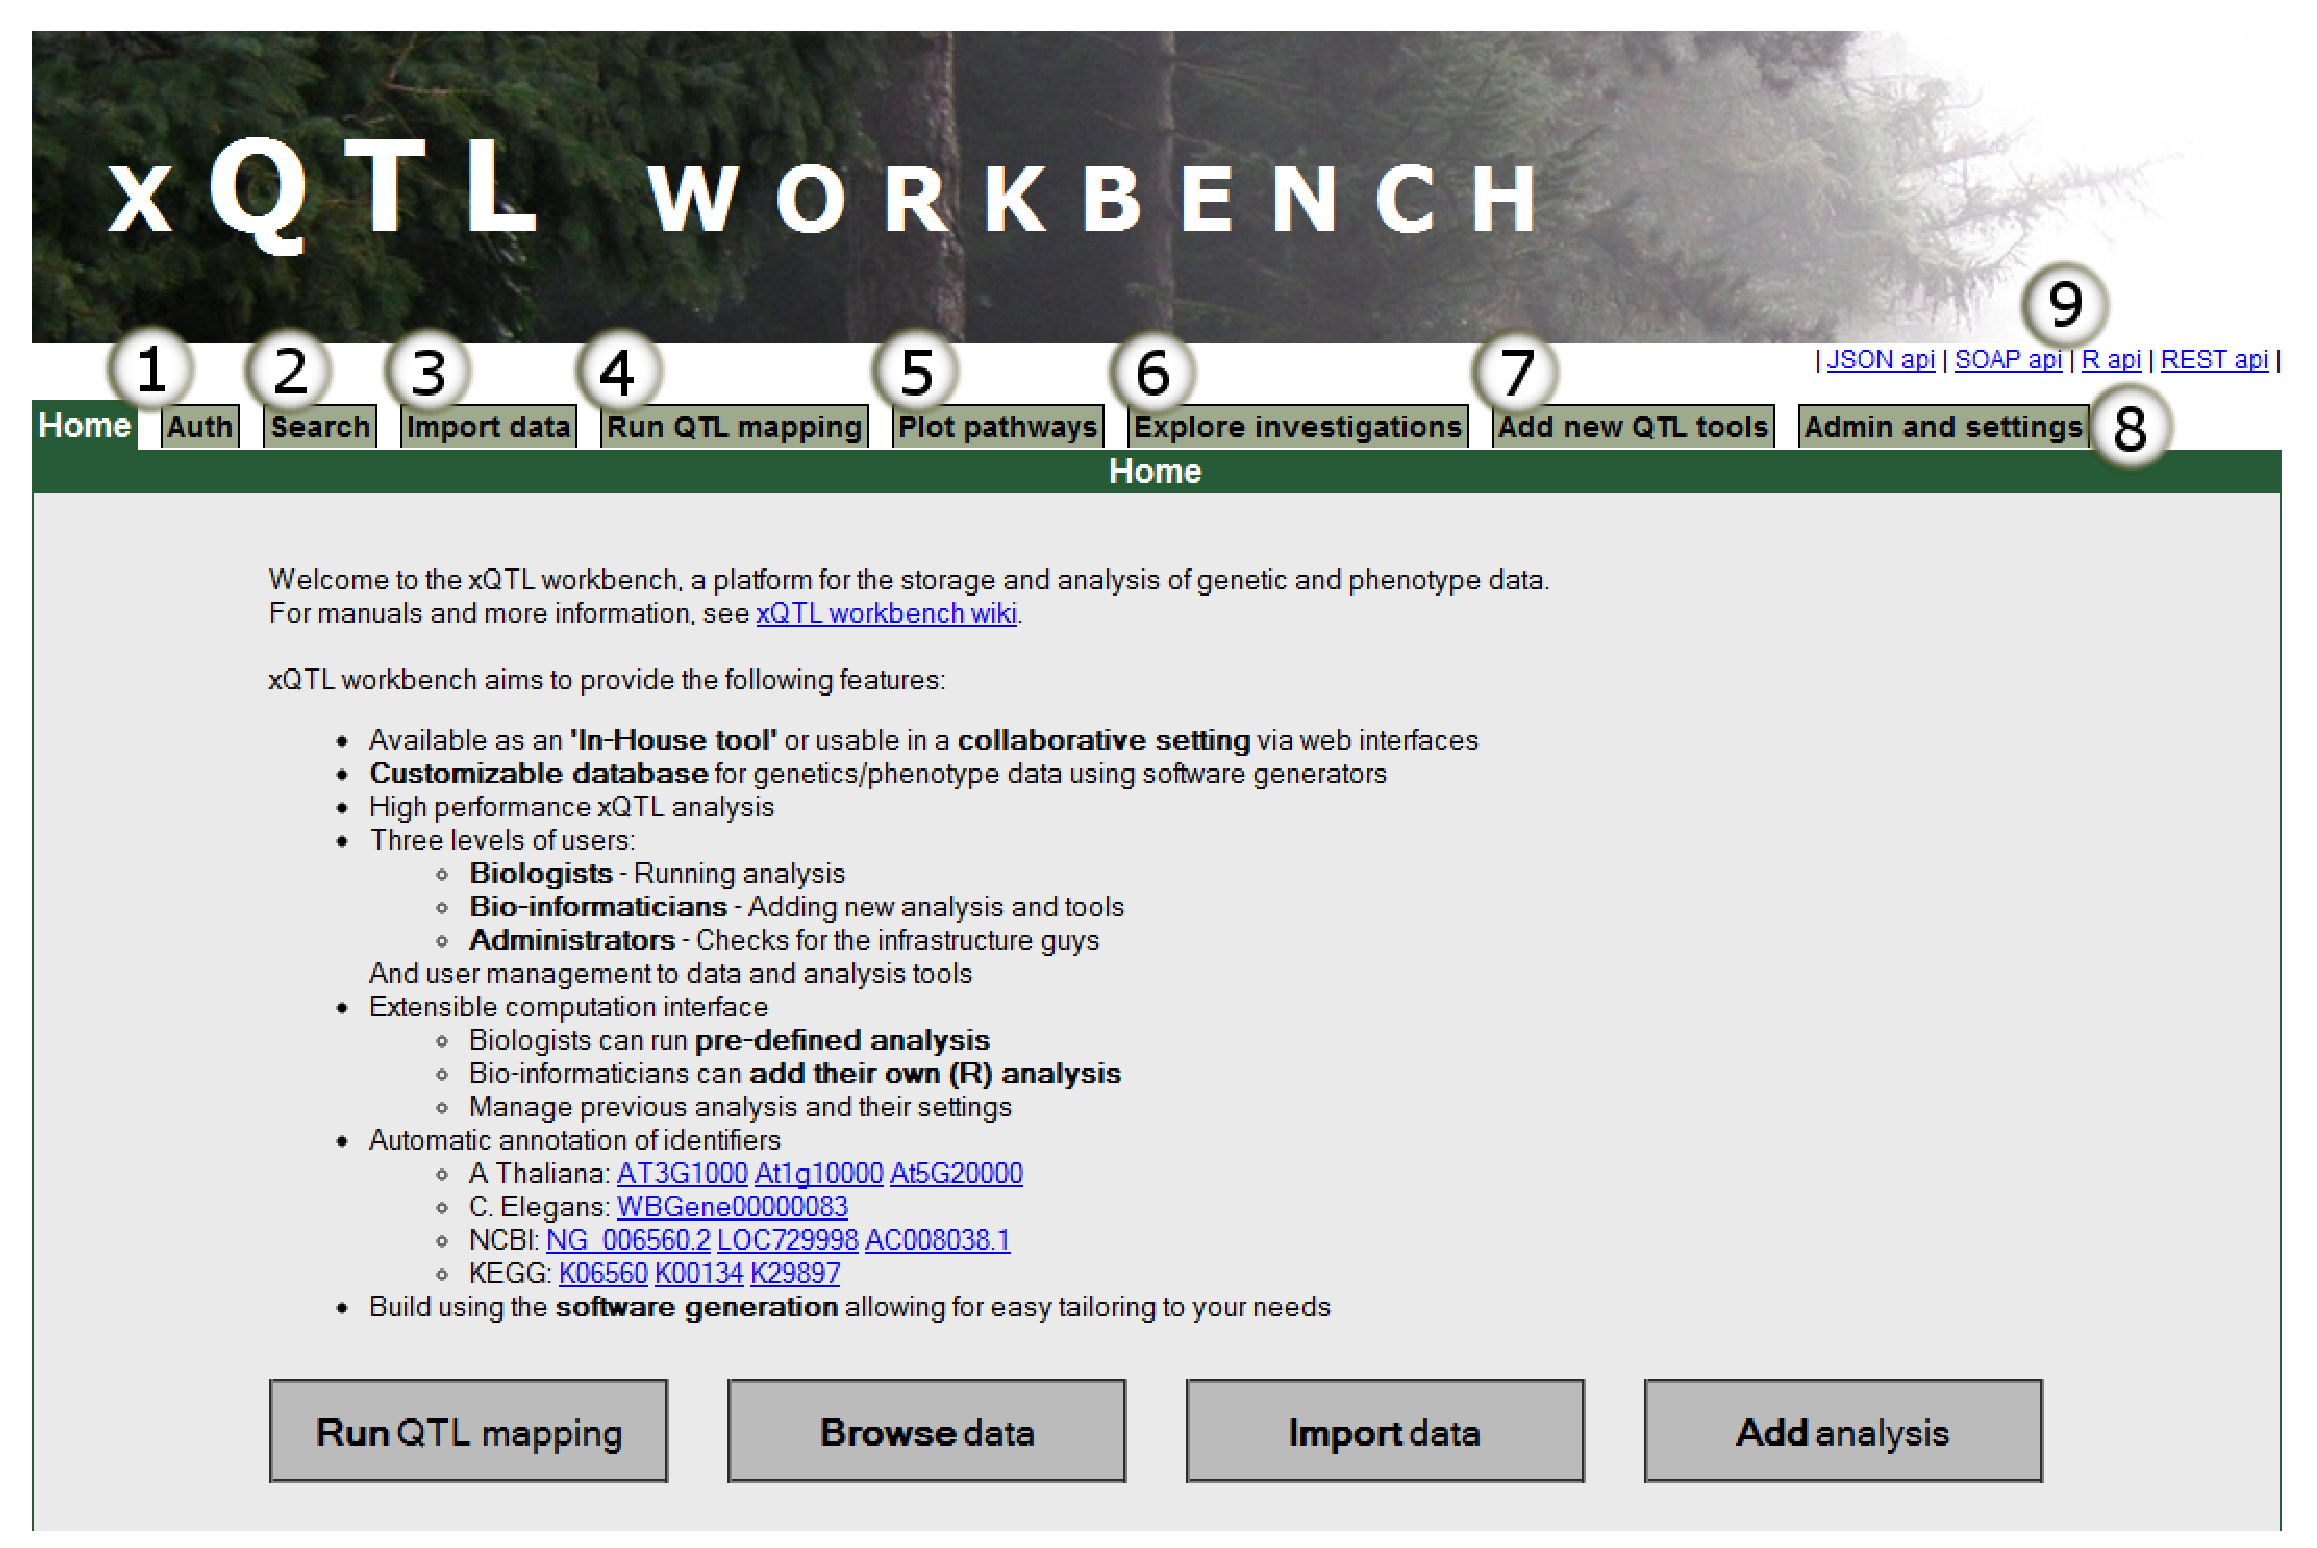
\includegraphics[width=0.9\textwidth]{eps/image_4_5.eps}
  \caption[Validation]{We systematically excluded datasets from our meta-analysis in order to determine the effect 
                       of sample size on the ability to detect significant interaction effects. The number of 
                       significant interaction effects dramatically decreases when the sample sizes becomes smaller. 
                       In general, lymphoid mediated \emph{cis}-eQTL effects are harder to detect than neutrophil mediated 
                       \emph{cis}-eQTL effects, due to their relatively small abundance in whole blood.  }
          \label{fig:fig4_5}
  \end{figure}

  Large sample sizes are essential in order to find cell-type-mediated \emph{cis}-eQTLs (Figure \ref{fig:fig4_5}): when we repeat our study on fewer samples 
  by systematically excluding more cohorts from our study, the number of significant cell-type-mediated eQTLs decreased 
  rapidly. This was particularly important for the lymphoid-mediated \emph{cis}-eQTLs, because myeloid cells are approximately twice as abundant 
  as lymphoid cells in whole blood. Consequently, detecting lymphoid-mediated \emph{cis}-eQTLs is more challenging than detecting myeloid-mediated 
  \emph{cis}-eQTLs. As whole blood eQTL data is easily collected, we were able to gather a sufficient sample size in order to detect 
  cell-type-mediated or -specific associations without requiring the actual purification of cell types. 

\begin{table}[h]
  \centering
  {\footnotesize
  \begin{tabular}{ | l | c | c | c | c | c | c | }
  {\bf Disease }          & {\bf SNPs} & {\bf AP} & {\bf \emph{cis}-eQTL SNPs} & {\bf NM} & {\bf Ratio} & {\bf P-value}\\
  \hline
  Crohn's disease         & 64   & 49 & 49 & 11 & 0.2895 & 0.0018\\
  IBD                     & 50   & 48 & 48 & 8 & 0.2000 & 0.0405\\
  Rheumatoid arthritis    & 34   & 27 & 27 & 3 & 0.1250 & 0.3846\\
  Multiple sclerosis      & 35   & 30 & 30 & 3 & 0.1111 & 0.4523\\
  Type 1 diabetes         & 27   & 21 & 21 & 2 & 0.1053 & 0.5242\\
  \end{tabular}
  }
  \caption[Disease enrichment]{Results of the different diseases tested for neutrophile mediated SNPs enrichment. AP = SNPs after pruning, NM = Number of 
  neutrophil mediated SNPs, P values reported are one tailed binomial pvalues. IDB = Inflammatory bowel disease}
  \label{tbl:tblDisease}
\end{table}


  \subsubsection{Software availability}
  The source code and documentation for this type of analysis are available as part of the eQTL meta-analysis pipeline at:\\
  \url{https://github.com/molgenis/systemsgenetics}\\
  Summary results are available from:\\
  \url{http://www.genenetwork.nl/celltype}

  \subsection{Discussion}
  Here we have shown that it is possible to infer in which cell-types \emph{cis}-eQTLs are operating, without 
  the actual need to sort cells. We used whole peripheral blood eQTL data of 5,683 unrelated samples. 
  By first estimating cell-type proportions and subsequent use of a G x E (i.e. the estimated cell-type 
  proportions) interaction model we were able to demonstrate that hundreds of \emph{cis}-eQTLs show stronger 
  effects in myeloid than lymphoid cell-types and vice versa. 

  Since we could subsequently replicate these results in 6 individual purified cell-type eQTL datasets 
  (two reflecting the myeloid and four reflecting the lymphoid lineage), this indicates G x E analyses 
  can provide important additional biological insights for many SNPs that have previously been found 
  to be associated with complex (molecular) traits. 

  However, two main criteria apply in order to identify such G x E effects: first, sample size should 
  be large. Although, to our knowledge, this is the largest eQTL study that has been conducted so-far 
  (5,683 samples), it is clear by sampling subsets of the participating cohorts (Figure 2), that more 
  G x E effects should be detectable with even larger sample sizes. Secondly, choosing the appropriate 
  environmental factor is essential in order to find convincing G x E effects: although we found 1,117 
  \emph{cis}-eQTLs that were mediated by myeloid or lymphoid cell-types, a recent G x E study that aimed to 
  detect \emph{cis}-eQTLs that were mediated by either gender or age (assessed in 5,254 samples) found only 
  five G x E effects that replicated in an independent cohort\cite{Whitlock:2005}. As such the choice of environmental 
  factor is crucial in order to find G x E interaction effects.

  Here, we have concentrated on identifying \emph{cis}-eQTLs that are preferentially operating in either 
  myeloid or lymphoid cell-types. We did not attempt to assess this for specialized cell-types within 
  the myeloid or lymphoid lineage. However, this is well possible if cell-counts are available for 
  these cell-types, or if these cell-counts can be estimated by using the expression levels of genes 
  that serve as proxies for those cell-counts. As such, identification of cell-type mediated eQTLs 
  for previously unstudied cell-types is possible, without the actual need to generate any new data. 
  However, it should be noted that these individual cell-types typically have a rather low abundance 
  within whole blood (e.g. natural killer cells only comprise ~2\% of all circulating white blood 
  cells). As a consequence, in order to have sufficient statistical power to identify eQTLs that are 
  mediated by these cell-types, very large whole blood eQTL sample-sizes are required (analogous to 
  the substantially lower number of identified lymphoid mediated \emph{cis}-eQTLs, as compared to the myeloid 
  mediated \emph{cis}-eQTLs, since neutrophils are twice as abundant as lymphoid cells in whole blood). 
  Additionally, such cell-types should show differences in abundance across different individuals, 
  rendering identification of \emph{cis}-eQTLs that are specific for certain cell-types impossible if those 
  cell-types have a near equal abundance in blood across each of the individuals.

  In order to improve statistical power to detect cell-type mediated eQTLs, we corrected the gene 
  expression for technical and batch effects (here we applied principal component analysis and removed 
  per cohort the 40 strongest principal components that affect gene expression). Such procedures are 
  commonly used when conducting \emph{cis}-eQTL mapping \cite{Lude:2011, Dubois:2010, Fu:2012, 
  Zhernakova:2013, Westra:2013, Lappalainen:2013}. Although this correction might diminish the 
  power to detect \emph{trans}-eQTLs \cite{Westra:2013}, this concern does not apply to our G x E \emph{cis}-eQTL study.

  We anticipate that with the (pending) availability of large RNA-seq based eQTL datasets, statistical 
  power to identify cell-type mediated eQTLs will improve further: since RNA-seq enables very accurate 
  gene expression level quantitation and is not limited to a set of preselected probes that interrogate 
  well known genes (as is the case for microarrays), the detection of genes that can serve as reliable 
  proxies for individual cell-types will improve. Secondly, using RNA-seq data, it is possible to 
  assess whether SNPs that affect the expression of non-coding transcripts, affect splicing \cite{Lappalainen:2013} or result 
  in alternative polyadenylation \cite{Zhernakova:2013} are mediated by specific cell-types.

  The method can be applied to eQTL data from any tissue, organ or whole organism, providing a computational alternative to sorting cells 
  or performing laser capture micro-dissection. The only prerequisite for our method is the availability of a relatively small training 
  dataset with cell count measurements in order to develop a reliable proxy for cell count measurements. Since the number of such training 
  datasets is rapidly increasing and meta-analyses have proven successful\cite{Lude:2011, Westra:2013}, our approach provides a cost-effective way to identify 
  cell-type-mediated or -specific associations, and it is likely to reveal major biological insights.

